%-------------------------------------------------------------------------------
% Document & Package declarations
%-------------------------------------------------------------------------------

\documentclass[a4paper, 10pt, conference]{ieeeconf}
\usepackage{graphicx}
\usepackage[colorlinks=true, allcolors=black]{hyperref}
\usepackage{tabularx}

%% Language and font encodings
\usepackage[english]{babel}
\usepackage[utf8x]{inputenc}
\usepackage[T1]{fontenc}

%% Useful packages
\usepackage{amsmath}
\usepackage{graphicx}
\usepackage[colorinlistoftodos]{todonotes}
% \usepackage[font=footnotesize,labelfont=bf]{caption}
% \usepackage[font=footnotesize,labelfont=bf]{subcaption}

%% Packages for displaying source code
\usepackage{listings}
% \usepackage[framed,numbered,autolinebreaks,useliterate]{mcode}

\usepackage{float}
\usepackage{longtable}

%% Packages for displaying source code
\usepackage[numbered,framed]{matlab-prettifier}
\usepackage{color}

%%*************************************************************************
%% Legal Notice:
%% This code is offered as-is without any warranty either expressed or
%% implied; without even the implied warranty of MERCHANTABILITY or
%% FITNESS FOR A PARTICULAR PURPOSE!
%% User assumes all risk.
%% In no event shall IEEE or any contributor to this code be liable for
%% any damages or losses, including, but not limited to, incidental,
%% consequential, or any other damages, resulting from the use or misuse
%% of any information contained here.
%%
%% All comments are the opinions of their respective authors and are not
%% necessarily endorsed by the IEEE.
%%
%% This work is distributed under the LaTeX Project Public License (LPPL)
%% ( http://www.latex-project.org/ ) version 1.3, and may be freely used,
%% distributed and modified. A copy of the LPPL, version 1.3, is included
%% in the base LaTeX documentation of all distributions of LaTeX released
%% 2003/12/01 or later.
%% Retain all contribution notices and credits.
%% ** Modified files should be clearly indicated as such, including  **
%% ** renaming them and changing author support contact information. **
%%
%% File list of work: IEEEtran.cls, IEEEtran_HOWTO.pdf, bare_adv.tex,
%%                    bare_conf.tex, bare_jrnl.tex, bare_jrnl_compsoc.tex,
%%                    bare_jrnl_transmag.tex
%%*************************************************************************

%-------------------------------------------------------------------------------
% Document Configuration
%-------------------------------------------------------------------------------

\begin{document}
\title{Pattern Recognition - Distance Metrics and Neural Networks}
\author{Michael~Hart (00818445) and
        Meng~Kiang~Seah (00699092)
\\
        Department of Electrical and Electronic Engineering, 
        Imperial College London, 
        SW7 2AZ
\\        
        E-mail: \{mh1613, mks211\}@imperial.ac.uk}
\date{\today}

%-------------------------------------------------------------------------------
% Plan on what to write
%-------------------------------------------------------------------------------

% See coursework instructions at: 
% https://bb.imperial.ac.uk/bbcswebdav/pid-1009576-dt-content-rid-3417906_1/courses/DSS-EE4_68-16_17/PRCoursework2.pdf

%-------------------------------------------------------------------------------
% Information Banner
%-------------------------------------------------------------------------------

\maketitle

%-------------------------------------------------------------------------------
% Abstract
%-------------------------------------------------------------------------------

\begin{abstract}
TODO ABSTRACT
\end{abstract}

%-------------------------------------------------------------------------------
% Introduction
%-------------------------------------------------------------------------------
\section{Introduction}

An introduction

%-------------------------------------------------------------------------------
% Distance Metrics
%-------------------------------------------------------------------------------
\section{Distance Metrics}

%-------------------------------------------------------------------------------
% K-means clustering
%-------------------------------------------------------------------------------
\section{K-means clustering}

%-------------------------------------------------------------------------------
% Neural Network
%-------------------------------------------------------------------------------
\section{Neural Network}

% Using Matlab Neural Network toolbox create a network, train and test with the wine data. Vary the parameters of the network to minimize the classification error. Report the observations and compare to the results from Q1 and Q2. Generate another random split of train/test/validation data and repeat the experiment. 

Neural networks are an often-used method of pattern recognition, due to their high accuracy, low error rates, and ease of use. They are flexible, and so can be adapted to most pattern recognition problems, such as the use of Convolutional Neural Networks (CNNs) in image recognition, an industry standard.

Neural networks take inspiration from biological neurons, which are interconnected and transmit information using sudden spikes in chemical levels. This is a process that can be simulated in software, including using MATLAB's neural network toolbox (NNT); this toolbox allows the creation, training and testing of various types of neural network.

This section tests the use of neural networks to minimise the Mean Squared Error (MSE), as a measure of the performance of the network. First the number of hidden neurons in a single layer fitting network is varied to test performance; results for a standard partition are shown in Table \ref{tbl:unmixed}. The fitting network was used as one of the most flexible types offered by the NNT, and most networks perform with near-optimal results using only a single hidden layer. The code used to generate these results is shown in the Appendix.

The two training algorithms with the minimum mean squared error (MSE) were determined; the results are shown in Figure \ref{fig:unmixed_full}. The effects of overfitting are clearly shown by the huge spike in both algorithms after around 100 hidden neurons. The comparison between the two algorithms is more clearly seen in Figure \ref{fig:unmixed_limited}, which limits the x-axis to 100 hidden neurons.

\begin{figure}[!ht]
    \centering
    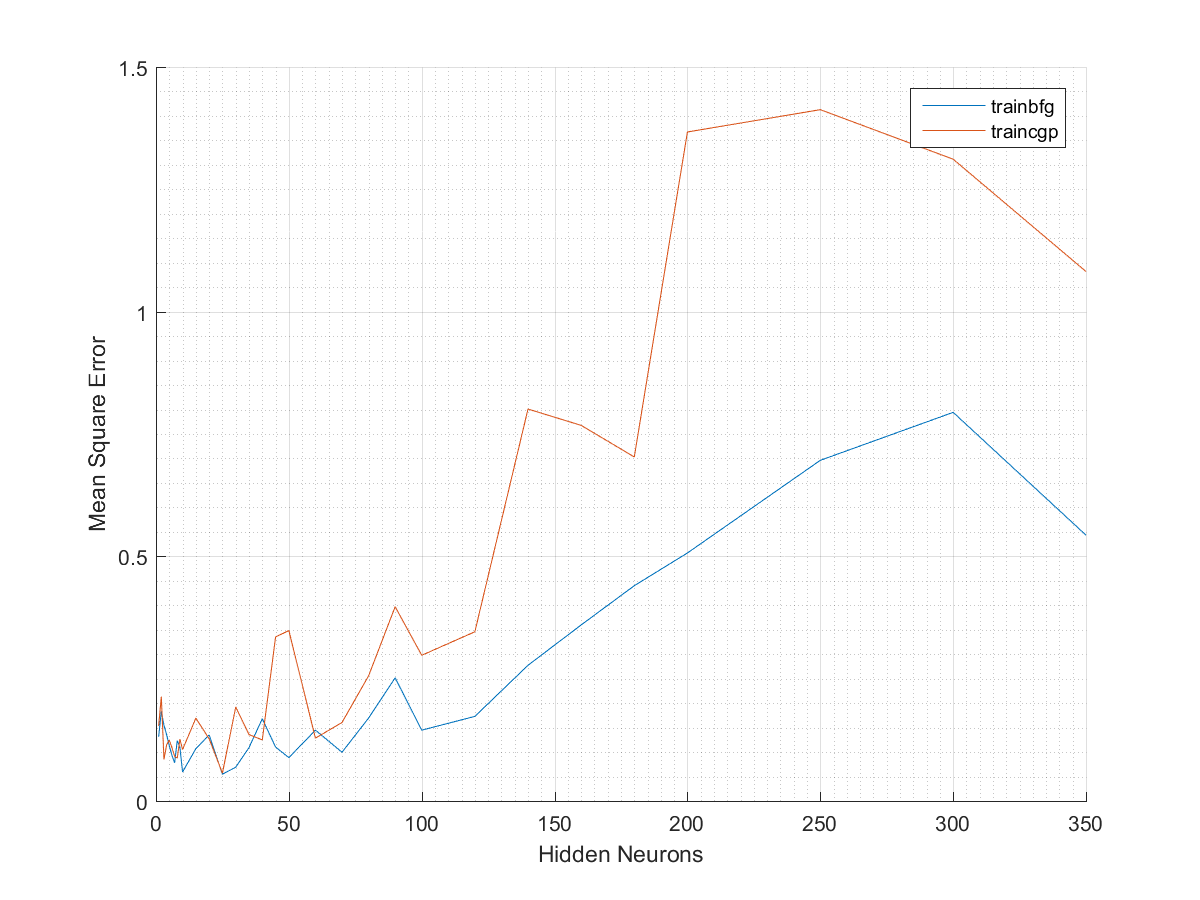
\includegraphics[width=\linewidth]{pic/unmixed_best_fullrange.png}
    \caption{MSE of best performing algorithms}
    \label{fig:unmixed_full}
\end{figure}

\begin{figure}[!ht]
    \centering
    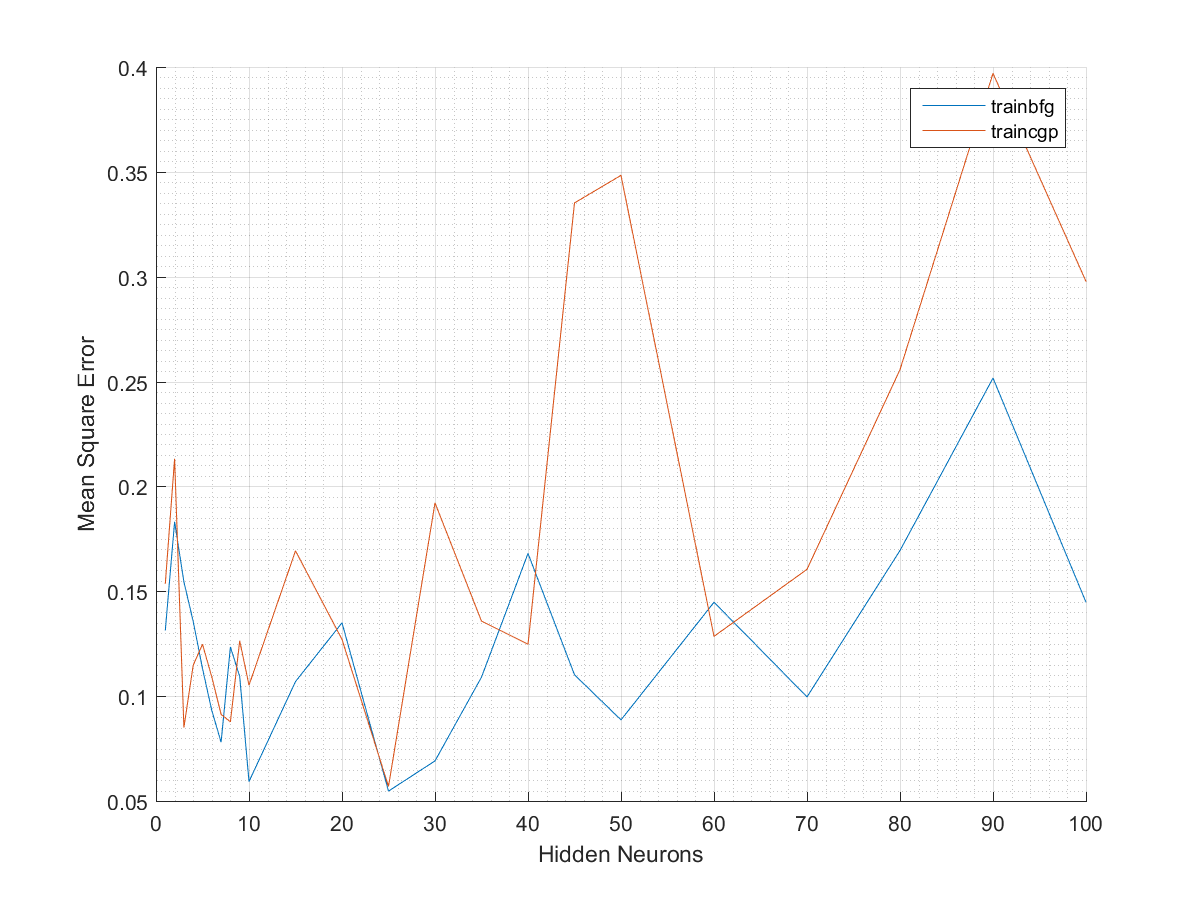
\includegraphics[width=\linewidth]{pic/unmixed_best_limited.png}
    \caption{MSE of best performing algorithms with limited axis}
    \label{fig:unmixed_limited}
\end{figure}

The graphs in the figures show a large variation in MSE between the lower numbers of hidden neurons, but overall there is a downward trend towards the apparent optimum of 25 hidden neurons, which indicates underfitting. After the lowest point, there is an upward trend, which indicates overfitting. Thus, the optimal number of nodes to use is likely between 10 and 50. The best performing algorithm from this data set is the \textit{trainbfg} algorithm.

However, although the standard partition provides an even comparison with other tasks, it does not provide the optimal method of training a network, which is to use a random partition. Therefore, the data in Table \ref{tbl:mixed} show the results of repartitioning with the same ratios, but in a random order. The graph is shown in Figure \ref{fig:mixed_limited}, already limited to 100 neurons due to the same overfitting effect as with the standard partition data.

With randomly partitioned data, the most effective training algorithm is \textit{trainlm} with 15 hidden neurons, but the graph shows that overall \textit{trainbr} is a more effective algorithm, even reducing the effects of overfitting. This is in contrast to the standard partition, which shows other algorithms to be more effective, but more surprisingly the random data shows a lower MSE overall. This implies that using random partitioning is a more effective method of training a neural network than a fixed or contiguous partitioning method; this is further backed up by the first 100\% classification accuracy results. The random partitioning data also shows that the optimum number of hidden neurons to use is between 10 and 50 neurons.

\begin{table}
\centering
\caption{Standard Partition - Hidden Neurons Comparison}
\label{tbl:unmixed}
\begin{tabular}{llllll}
\hline
\textbf{Algorithm} & \textbf{Neurons} & \textbf{Time to Train (s)} & \textbf{Accuracy} & \textbf{MSE} \\ \hline
trainbfg & 15 & 0.15658 & 0.9 & 0.10695 \\ \hline 
trainbfg & 20 & 0.23614 & 0.8 & 0.13496 \\ \hline 
trainbfg & 25 & 0.82571 & 0.95 & 0.054725 \\ \hline 
trainbfg & 30 & 0.76897 & 0.95 & 0.069127 \\ \hline 
trainbfg & 35 & 0.70948 & 0.85 & 0.10906 \\ \hline

traincgp & 15 & 0.066146 & 0.825 & 0.16928 \\ \hline 
traincgp & 20 & 0.09904 & 0.875 & 0.12706 \\ \hline 
traincgp & 25 & 0.10311 & 0.95 & 0.05694 \\ \hline 
traincgp & 30 & 0.075015 & 0.85 & 0.19212 \\ \hline 
traincgp & 35 & 0.11164 & 0.85 & 0.13576 \\ \hline 
\end{tabular}
\end{table}

\begin{figure}[!ht]
    \centering
    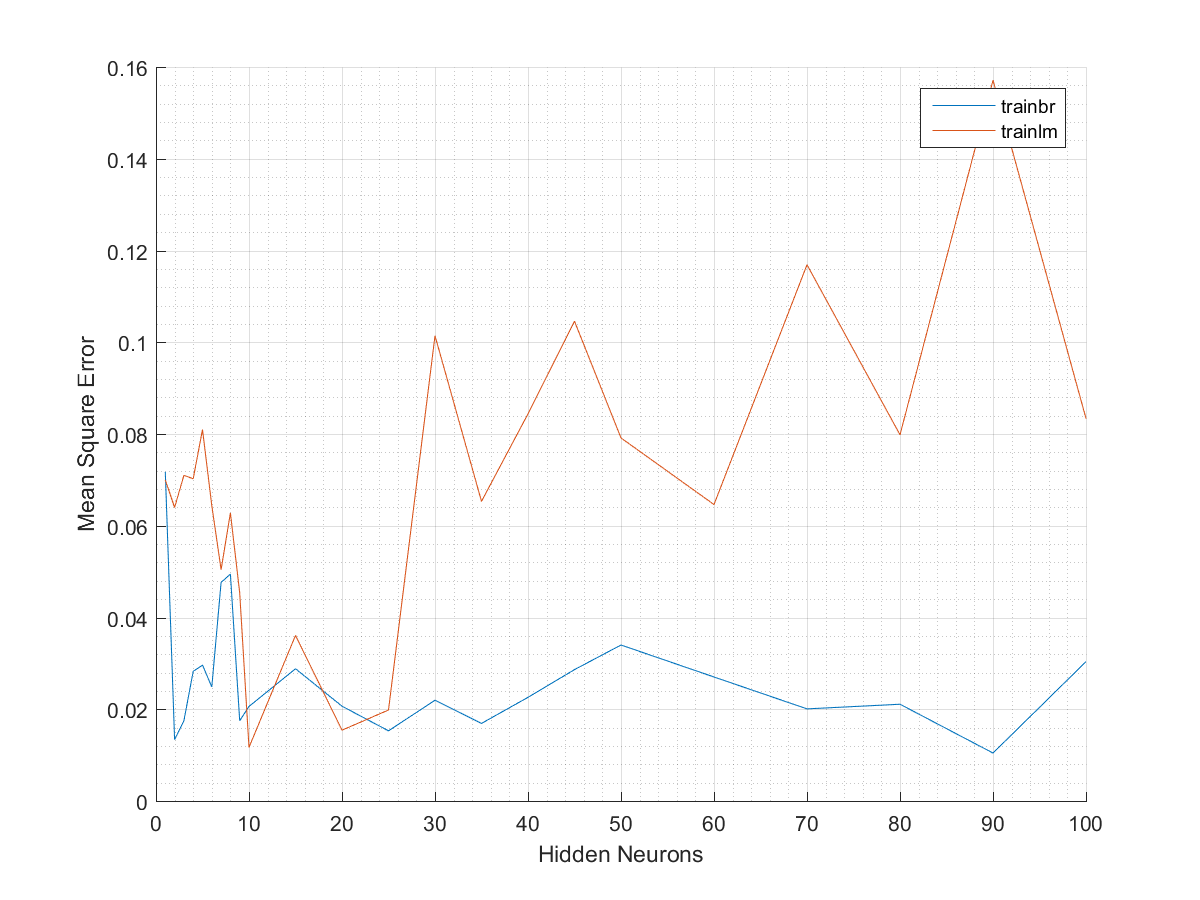
\includegraphics[width=\linewidth]{pic/mixed_best_limited.png}
    \caption{MSE of best performing algorithms with limited axis with random partition}
    \label{fig:mixed_limited}
\end{figure}

\begin{table}
\centering
\caption{Random Partition - Hidden Neurons Comparison}
\label{tbl:mixed}
\begin{tabular}{llllll}
\hline
\textbf{Algorithm} & \textbf{Neurons} & \textbf{Time to Train (s)} & \textbf{Accuracy} & \textbf{MSE} \\ \hline
trainbr & 15 & 5.8827 & 0.975 & 0.028823 \\ \hline 
trainbr & 20 & 8.1333 & 0.975 & 0.020667 \\ \hline 
trainbr & 25 & 14.6828 & 1 & 0.015294 \\ \hline 
trainbr & 30 & 20.2646 & 0.975 & 0.021972 \\ \hline 
trainbr & 35 & 28.5412 & 1 & 0.016915 \\ \hline 

trainlm & 15 & 0.0657085 & 0.95 & 0.036084 \\ \hline 
trainlm & 20 & 0.0607793 & 1 & 0.015435 \\ \hline 
trainlm & 25 & 0.0679456 & 1 & 0.019838 \\ \hline 
trainlm & 30 & 0.0846978 & 0.85 & 0.10142 \\ \hline 
trainlm & 35 & 0.0921787 & 0.975 & 0.065321 \\ \hline 
\end{tabular}
\end{table}

% TODO Decide whether to visualise matlab's performance stuff and what-have-you. Need to force-add image of network I already have as well as concatenating all data together for the testing phase

The examination of neural networks thus far has shown that the most effective number of neurons for a single layer fitting network is in the range of 10-50 approximately. To further minimise the MSE in neural networks, multiple types of network were investigated, simultaneously with the number of layers per network. The code for this may be found in the Appendix; the results with minimum MSE are shown in Tables \ref{tbl:unmixed_networks} and \ref{tbl:mixed_networks}, representing standard and random partition results respectively.

% Tables of interesting data from network and layers comparison
\begin{table}
\centering
\caption{Standard Partition - Network and Layer Comparison}
\label{tbl:unmixed_networks}
\begin{tabular}{llllll}
\hline
\textbf{Network} & \textbf{Algorithm} & \textbf{Layers} & \textbf{Neurons} & \textbf{$T_{train}$} & \textbf{MSE} \\ \hline
pattern & trancgf & 3 & 20 & 0.086992 & 0.034907 \\ \hline
pattern & trainscg & 3 & 20 & 0.065218 & 0.040891 \\ \hline
pattern & trainlm & 2 & 10 & 0.083229 & 0.042546 \\ \hline
pattern & traincgp & 1 & 40 & 0.053625 & 0.0484 \\ \hline
fit & trainbfg & 2 & 30 & 38.0862 & 0.050361 \\ \hline
\end{tabular}
\end{table}

\begin{table}
\centering
\caption{Random Partition - Network and Layer Comparison}
\label{tbl:mixed_networks}
\begin{tabular}{llllll}
\hline
\textbf{Network} & \textbf{Algorithm} & \textbf{Layers} & \textbf{Neurons} & \textbf{$T_{train}$} & \textbf{MSE} \\ \hline
fit & trainbr & 2 & 10 & 6.7953 & 0.01676 \\ \hline
fit & trainbr & 1 & 10 & 0.9048 & 0.01691 \\ \hline
pattern & trainlm & 3 & 25 & 4.2124 & 0.01707 \\ \hline
pattern & trainscg & 3 & 15 & 0.0668& 0.01846 \\ \hline
feedforward & traincgp & 3 & 15 & 0.1105 & 0.01892 \\ \hline
\end{tabular}
\end{table}

The standard partition shows that a different type of network has proved most effective. \textit{Patternnet} is the network that is intended for use in pattern recognition applications, such as this one. However, the MSE of standard partition is still greater than that attained by randomly partitioned data, which uses a fitting network with \textit{trainbr} algorithm as the most effective method, matching very closely with the results of the previous data set. In fact, the previous set of data showed a lower MSE using \textit{trainbr} with a single layer of 25 neurons, which was not investigated in the latter data set due to the large amount of training time required. 

Overall, the data shown in this section suggests that the most effective method of minimising error from a neural network is to randomly partition the data, and use a fitting network of a single layer of 25 neurons with the \textit{trainbr} training algorithm. It is possible that more layers of 25 neurons would increase accuracy, but at the cost of training and test time with a minimal decrease in MSE.

% TODO compare MSE and accuracy with other tasks

%-------------------------------------------------------------------------------
% Conclusion
%-------------------------------------------------------------------------------
\section{Conclusion}

A conclusion \cite{pca}. 

%-------------------------------------------------------------------------------
% References
%-------------------------------------------------------------------------------
\bibliographystyle{unsrt}
\bibliography{pr_refs}

%-------------------------------------------------------------------------------
% Appendix(ces)
%-------------------------------------------------------------------------------
\onecolumn
\section{Appendix} \label{sec:appendix}

\subsection*{Test set code for Task 3}
\lstinputlisting[style=Matlab-editor]{src/task3_all.m}
\newpage

\subsection*{Making and testing of neural network}
\lstinputlisting[style=Matlab-editor]{src/make_test_nn.m}
\newpage

\subsection*{Test code for various layers/networks for Task 3}
\lstinputlisting[style=Matlab-editor]{src/task3_networks.m}
\newpage

\end{document}